\section{INTRODUCTION}

As a research university, we offer undergraduate students opportunities to work on major research projects, with different students rotating in and out, semester to semester. For those more interested in the applied disciplines (e.g. engineering, journalism, law, business, social work) there are fewer such opportunities. Our innovation is a course design which would give the ``major project" experience in an experiential form, for students in the applied disciplines. We call it multi-semester/multi-cohort. 

\begin{figure}[!ht]
  \centering
  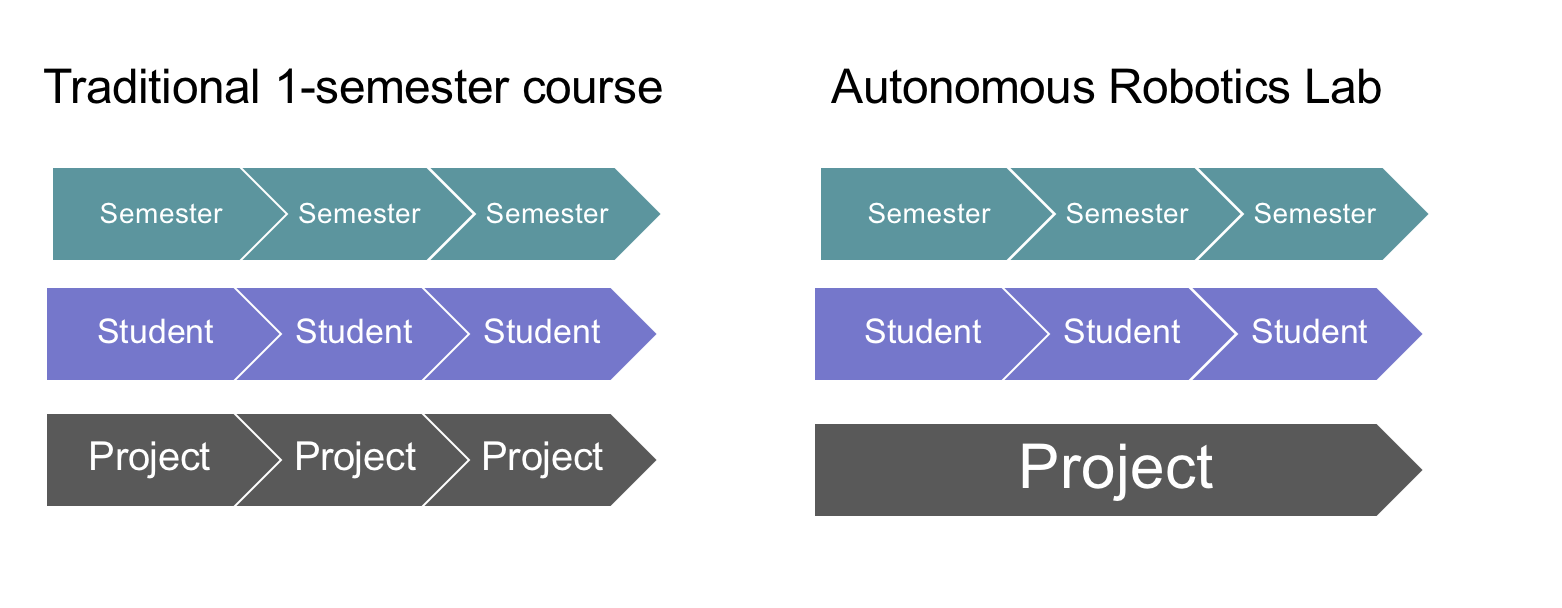
\includegraphics[width=\columnwidth,height=6cm]{diag1}
  \caption{Multi Semester/Multi Cohort structure}
  \label{fig:diag1}
\end{figure}

``Multi-semester" because the project will not (cannot) be completed in one semester, and ``multi-cohort" because the set of students working on it changes from semester to semester. We wanted to see whether it would work, and learn how to organize things to allow each semester’s cohort to pass knowledge to the next one in an efficient way, and how assessment would work.

We are inspired by the idea of a ``BHAG" (Big Hairy Audacious Goal), conceptualized in \cite{Collins}. Collins and Porras describe this mouthful term as follows:

\begin{quote}
``We found in our research that visionary companies often use bold missions --- BHAGs, shorthand for Big, Hairy, Audacious Goals] --- as a powerful way to stimulate progress.... A true BHAG is clear and compelling, serves as a unifying focal point of effort, and acts as a catalyst for team spirit. It has a clear finish line, so the organization can know when it has achieved the [goal] A BHAG engages people --- it reaches out and grabs them. It is tangible, energizing, highly focused.\cite{Collins}"
\end{quote}

For our course, our BHAG is "Campus Rover", a robot that can travel both indoors and outdoors on campus to deliver packages from an office in one building to an office in another building.After our first semester pilot, we made changes and refinements in the program, and we are now in our second semester. This paper describes the curriculum and how it has evolved, and explores what works and does not.

